\subsection{Resultados do treinamento com o \textit{dataset Galhardi} (Português) usando o Modelo \textit{BERTimbau Base}}

Os resultados do treinamento com o \textit{dataset Galhardi} em português utilizando o modelo \textit{BERTimbau Base} mostram uma acurácia média variando de 59.35\% a 63.43\%. A acurácia mais alta foi alcançada com 80\% dos dados de treinamento. Apesar de a acurácia média ser menor em comparação com os modelos de inglês e espanhol que serão exibidos em após os resultados em portugês.

\begin{table}[h!]
\centering
\resizebox{\columnwidth}{!}{%
\begin{tabular}{|p{0.25\textwidth}|p{0.1\textwidth}|p{0.1\textwidth}|p{0.4\textwidth}|p{0.1\textwidth}|p{0.1\textwidth}|p{0.1\textwidth}|}
    \hline
    \textbf{Percentual de dados para o treinamento} & \textbf{Qtd. Treino} & \textbf{Qtd. Teste} & \textbf{Pesos [Fator 1, Fator 2, Fator 3]} & \textbf{EQM} & \textbf{EMA} & \textbf{Acurácia média} \\
    \hline
     60\% & 14026 & 9352 & [0.6540, 0.2649, 0.2679] & 0.5211 & 0.5284 & 59.35\% \\
    \hline
     70\% & 16364 & 7014 & [0.6064, 0.2940, 0.2973] & 0.5165 & 0.5262 & 61.46\% \\
    \hline
     80\% & 18702 & 4676 & [0.5772, 0.2574, 0.3362] & 0.5385 & 0.5375 & 63.43\% \\
    \hline
     90\% & 21040 & 2338 & [0.4971, 0.2798, 0.4261] & 0.5950 & 0.5686 & 62.26\% \\
    \hline
\end{tabular}%
}
\caption{Resultados de Regressão para Diferentes Percentuais de Treino com o \textit{dataset Galhardi} (Português) usando o Modelo \textit{BERTimbau Base}}
\label{tab:resultados_regressao_portugues_base}
\end{table}

Nos gŕafico das Figuras \ref{figure:44}, \ref{figure:45}, \ref{figure:46} e \ref{figure:47}  é possível ver uma concetração dos dados na faixa de 40\% até 60\%, com uma queda dessa faixa mais notável na \ref{figure:47}.


\begin{figure}[h!]
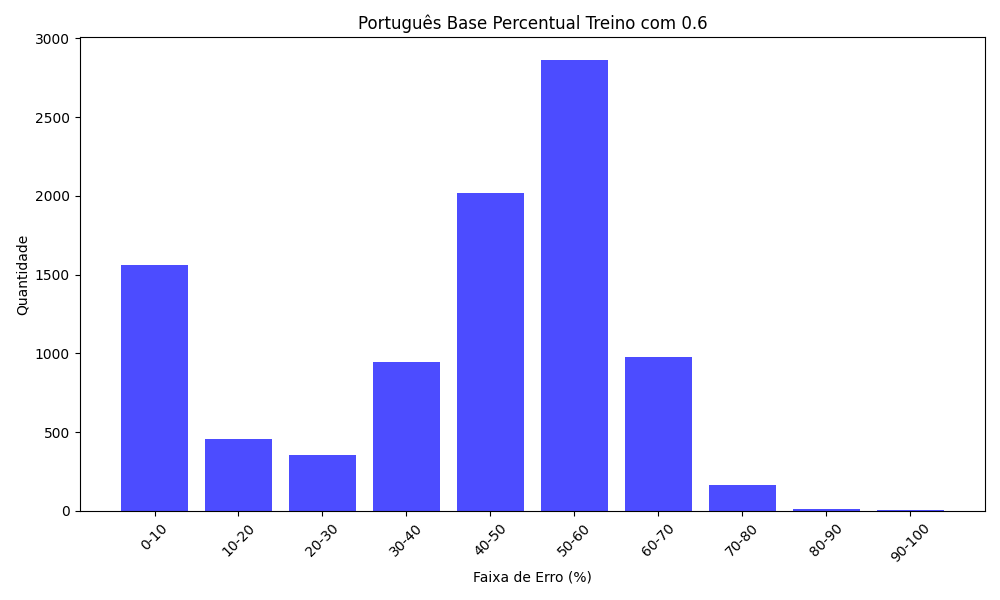
\includegraphics[width=\textwidth]{img/grafsPort/Português Base Percentual Treino com 0.6_quantidade.png}
\caption{Quantidade de respostas por faixas de erro percentual dos testes com 40\% do \textit{dataset Galhardi} (Português) usando o Modelo \textit{BERTimbau Base})}\label{figure:44}
\end{figure}

\begin{figure}[h!]
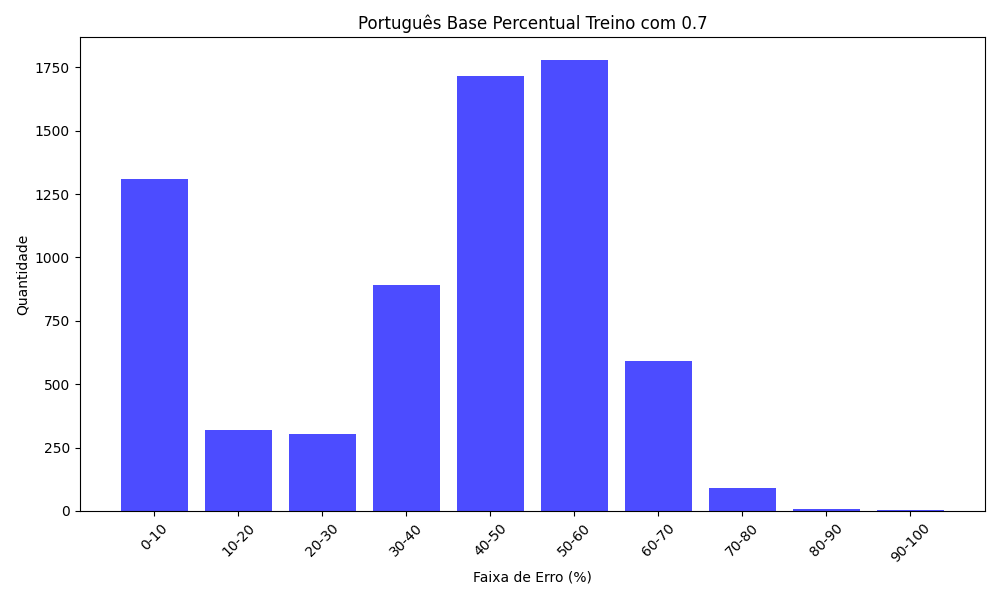
\includegraphics[width=\textwidth]{img/grafsPort/Português Base Percentual Treino com 0.7_quantidade.png}
\caption{Quantidade de respostas por faixas de erro percentual dos testes com 30\% do \textit{dataset Galhardi} (Português) usando o Modelo \textit{BERTimbau Base})}\label{figure:45}
\end{figure}

\begin{figure}[h!]
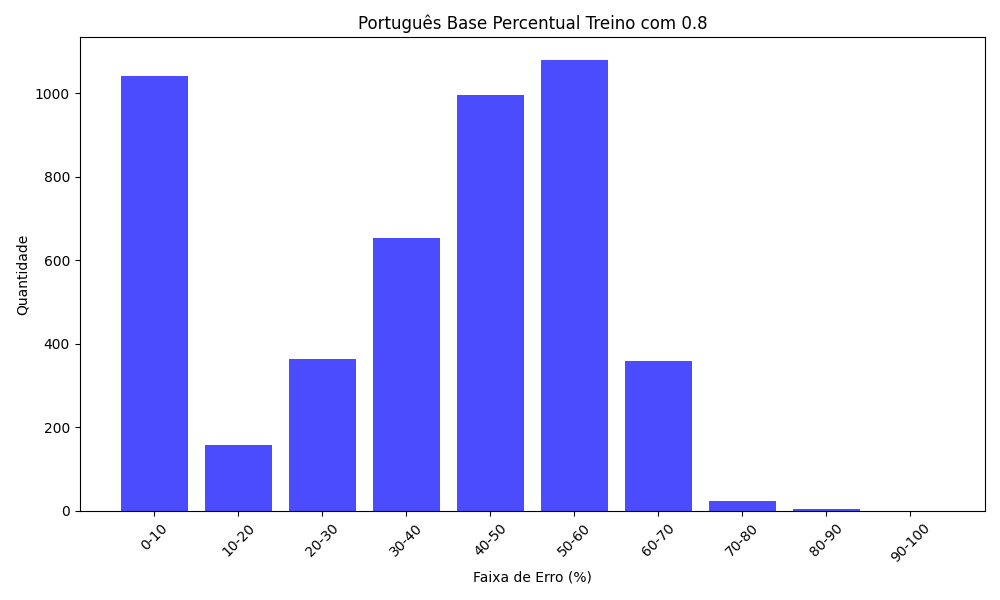
\includegraphics[width=\textwidth]{img/grafsPort/Português Base Percentual Treino com 0.8_quantidade.png}
\caption{Quantidade de respostas por faixas de erro percentual dos testes com 20\% do \textit{dataset Galhardi} (Português) usando o Modelo \textit{BERTimbau Base})}\label{figure:46}
\end{figure}

\begin{figure}[h!]
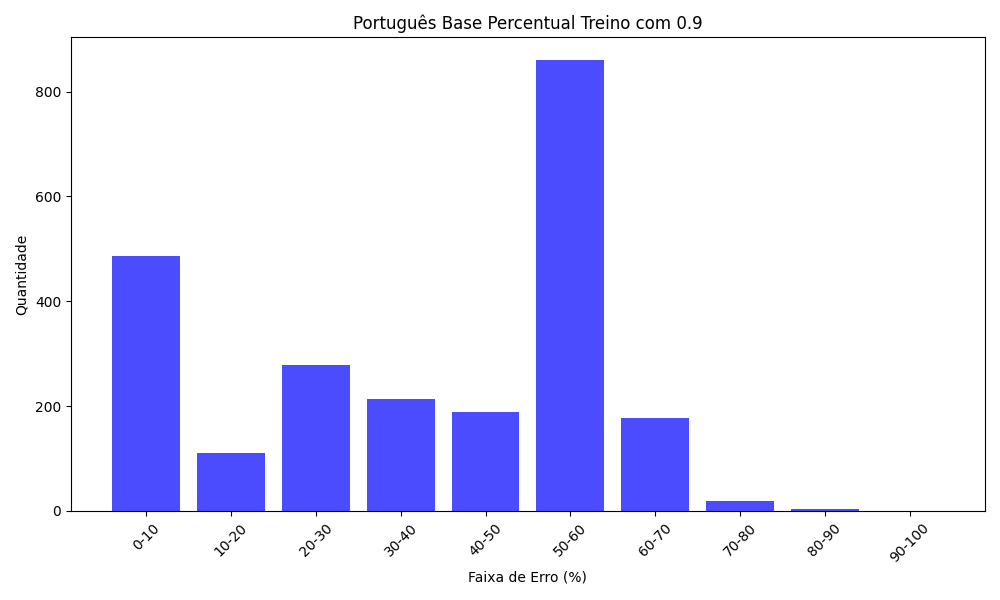
\includegraphics[width=\textwidth]{img/grafsPort/Português Base Percentual Treino com 0.9_quantidade.png}
\caption{Quantidade de respostas por faixas de erro percentual dos testes com 10\% do \textit{dataset Galhardi} (Português) usando o Modelo \textit{BERTimbau Base})}\label{figure:47}
\end{figure}

\FloatBarrier

%--------------------------------------------------

\subsection{Resultados do treinamento com o \textit{dataset Galhardi} (Português) usando o Modelo \textit{BERTimbau Large}}

Os resultados para o \textit{dataset Galhardi} em português utilizando o modelo \textit{BERTimbau Large} indicam uma acurácia média variando entre 55.4\% e 59.83\%. A acurácia mais alta foi obtida com 80\% dos dados de treinamento. Embora a acurácia média seja menor do que a observada com o modelo \textit{BERTimbau Base}, os valores de EQM e EMA sugerem que o modelo \textit{BERTimbau Large} pode precisar de mais ajustes para alcançar um desempenho superior em tarefas de linguagem natural em português, pelo menos quando usado na tarefa de avaliar similaridade semântica.

\begin{table}[h!]
\centering
\resizebox{\columnwidth}{!}{%
\begin{tabular}{|p{0.25\textwidth}|p{0.1\textwidth}|p{0.1\textwidth}|p{0.4\textwidth}|p{0.1\textwidth}|p{0.1\textwidth}|p{0.1\textwidth}|}
    \hline
    \textbf{Percentual de dados para o treinamento} & \textbf{Qtd. Treino} & \textbf{Qtd. Teste} & \textbf{Pesos [Fator 1, Fator 2, Fator 3]} & \textbf{EQM} & \textbf{EMA} & \textbf{Acurácia média} \\
    \hline
    60\% & 14026 & 9352 & [0.7045, 0.2960, 0.5349] & 0.5230 & 0.5318 & 55.4\% \\
    \hline
    70\% & 16364 & 7014 & [0.6538, 0.3434, 0.5882] & 0.5201 & 0.5317 & 58.14\% \\
    \hline
    80\% & 18702 & 4676 & [0.6335, 0.3061, 0.6643] & 0.5438 & 0.5443 & 59.83\% \\
    \hline
    90\% & 21040 & 2338 & [0.5673, 0.3484, 0.8416] & 0.6037 & 0.5765 & 57.91\% \\
    \hline
\end{tabular}%
}
\caption{Resultados de Regressão para Diferentes Percentuais de Treino com o \textit{dataset Galhardi} (Português) usando o Modelo \textit{BERTimbau Large}}
\label{tab:resultados_regressao_portugues_large}
\end{table}

Nos gŕafico das Figura \ref{figure:34} é possível ver uma concetração dos dados na faixa de 50\% até 70\%, embora na Figura \ref{figure:37} o erro pareça menor, ainda é possível notar que esse faixa possui mais concentração que as outras.

\begin{figure}[h!]
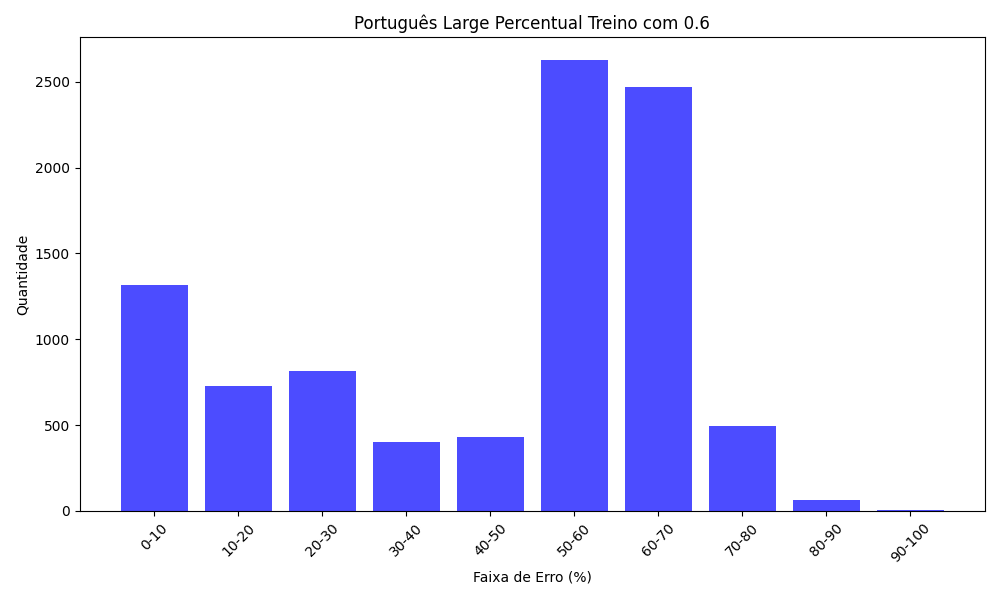
\includegraphics[width=\textwidth]{img/grafsPort/Português Large Percentual Treino com 0.6_quantidade.png}
\caption{Quantidade de respostas por faixas de erro percentual dos testes com 40\% do \textit{dataset Galhardi} (Português) usando o Modelo \textit{BERTimbau Large})}\label{figure:34}
\end{figure}

\begin{figure}[h!]
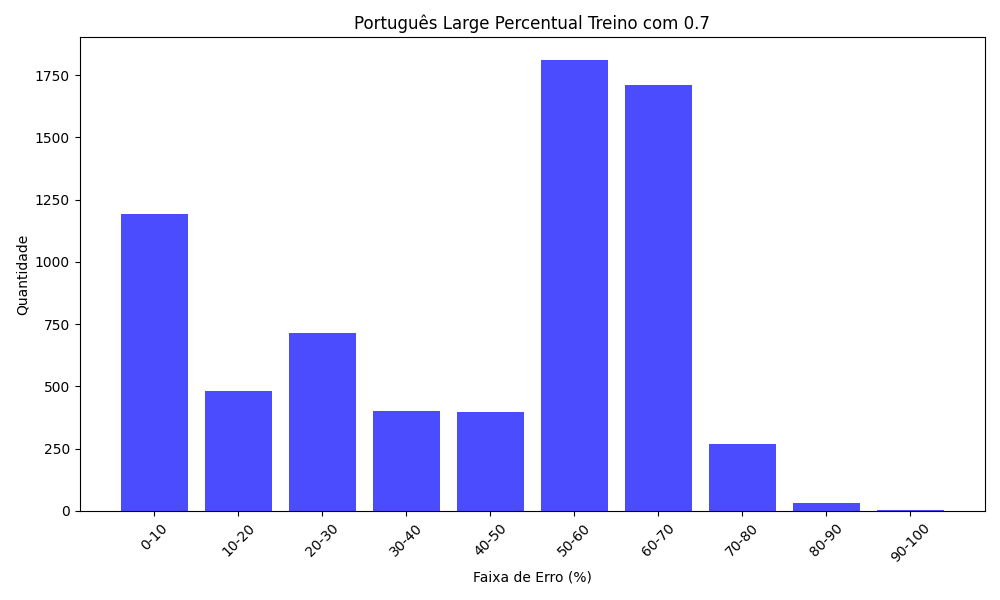
\includegraphics[width=\textwidth]{img/grafsPort/Português Large Percentual Treino com 0.7_quantidade.png}
\caption{Quantidade de respostas por faixas de erro percentual dos testes com 30\% do \textit{dataset Galhardi} (Português) usando o Modelo \textit{BERTimbau Large})}\label{figure:35}
\end{figure}

\begin{figure}[h!]
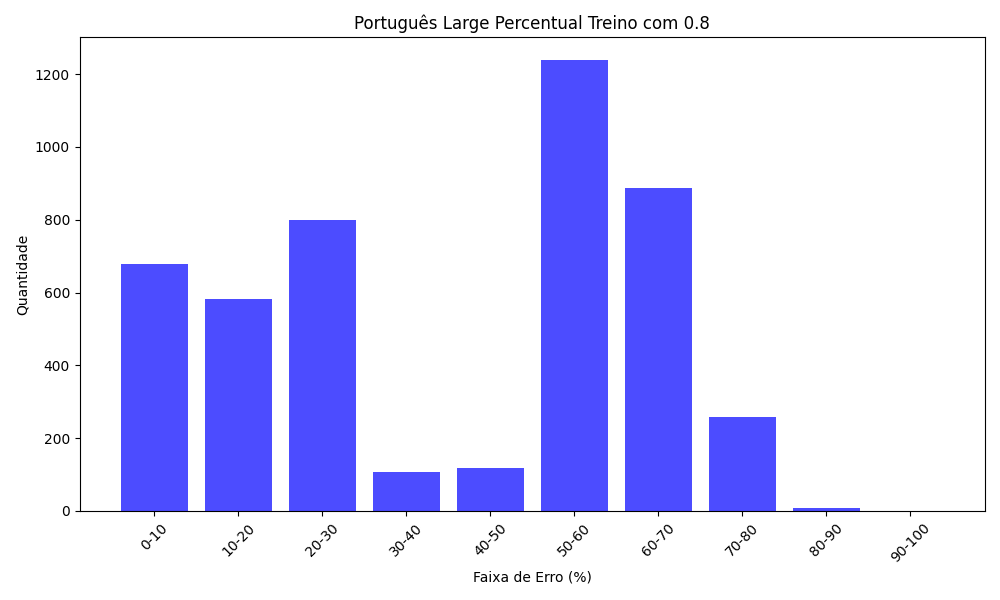
\includegraphics[width=\textwidth]{img/grafsPort/Português Large Percentual Treino com 0.8_quantidade.png}
\caption{Quantidade de respostas por faixas de erro percentual dos testes com 20\% do \textit{dataset Galhardi} (Português) usando o Modelo \textit{BERTimbau Large})}\label{figure:36}
\end{figure}

\begin{figure}[h!]
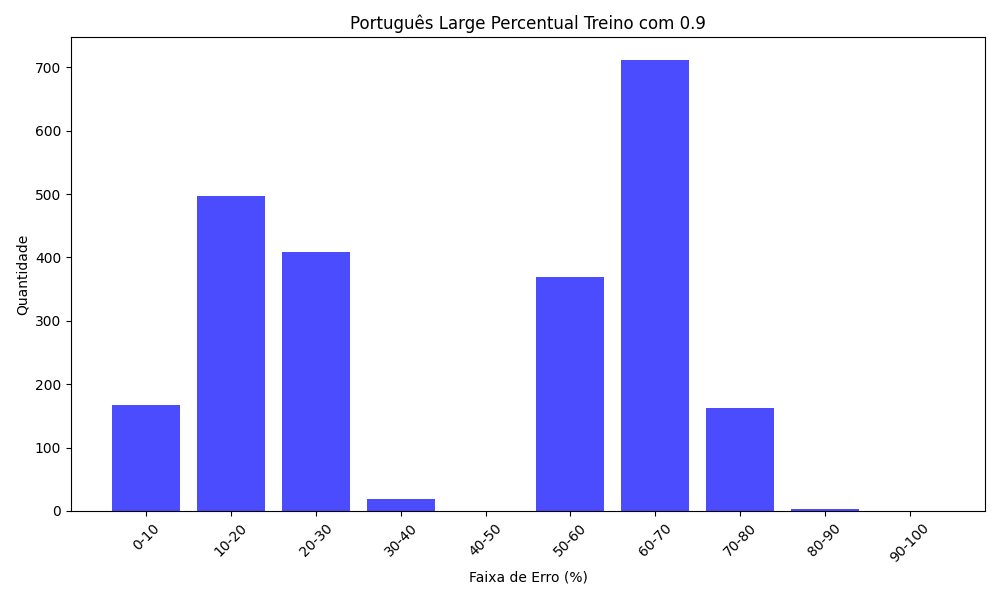
\includegraphics[width=\textwidth]{img/grafsPort/Português Large Percentual Treino com 0.9_quantidade.png}
\caption{Quantidade de respostas por faixas de erro percentual dos testes com 10\% do \textit{dataset Galhardi} (Português) usando o Modelo \textit{BERTimbau Large})}\label{figure:37}
\end{figure}

\FloatBarrier